%====================================================================================
\section[Censurado y truncado]{Modelos de regresión censurados y truncados}
%====================================================================================


\begin{frame}{A modo de repaso}
	\begin{itemize}
		\item Usamos probit y logit para una respuesta binaria.
		\item Usamos Tobit para una solución de esquina (``corner solution outcome'')   
	\end{itemize}
	Usualmente otro rasgo de los datos cae en la misma categor\'{i}a de variables restringidas por un valor; en este caso estamos hablando de una variable censurada.
\end{frame}
%---------------------------------------------------
\begin{frame}{El modelo de datos censurados}
	¿Cómo surge una variable censurada?
		\begin{itemize}
			\item \textit{Survey design}. Es un caso de missing data (en la variable dependiente). Por ejemplo, demanda por tickets en eliminatorias para los últimos cupos al mundial.
			\item En algunos casos restricciones institucionales (Wooldridge).	   
		\end{itemize}
\end{frame}
%---------------------------------------------------
\begin{frame}{El modelo de datos censurados}
	\begin{itemize}
		\item ¿Cúal es el rasgo del modelo de variable censurada? Las unidades son observables y proveen información de las variables independientes ($X$'s); pero la información sobre la variable dependiente esta ausente (variable omitida). Es de conocimiento el valor de corte. Este valor puede ser superior (\textit{right censoring}) o inferior (\textit{left censoring}).
		\item Unidades escogen opciones como ``mas de 50 000 dólares'' ( threshold); se observan datos menos de 50 000 dólares.
		\item La misma respuesta del \textit{threshold} para muchas observaciones $i$.
	\end{itemize}
\end{frame}
%---------------------------------------------------
\begin{frame}
	\begin{figure}[htbp]
		\hspace*{+1cm} 
		\centering
			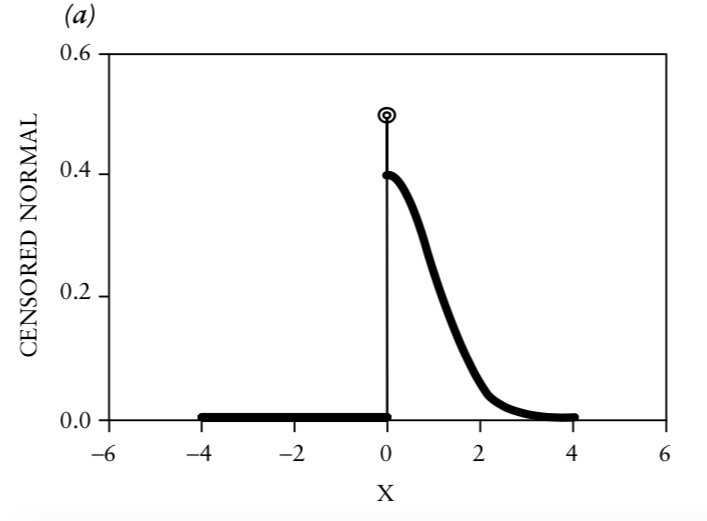
\includegraphics[width=0.65\linewidth]{fig/censored-model} % requires the graphicx package
		\label{censored}
		\caption{Source: Heij et. al 2004 ``Econometric Methods with Applications in Business and Economics''}
	\end{figure} 
\end{frame}
%---------------------------------------------------
\begin{frame}{El modelo de datos censurados}
	El modelo censurado puede expresarse de la siguiente manera:
		\begin{align}
			y_i=& \boldsymbol{x_i\beta}+u_i, \ u_i |  \ x_i, c_i \ \sim Normal(0,\sigma^2) \\
			w_i=&\min(y_i,c_i)
		\end{align}
	$u_i$ is independent of $c_i$
\end{frame}
%---------------------------------------------------
\begin{frame}
	¿Cuál es el problema de estimar este modelo por OLS? Las razones son similares como en el caso del modelo TOBIT.
		\begin{itemize}
			\item Los $\beta$'s son inconsistentes.	
		\end{itemize}
	Sin embargo existe un punto importante; en el modelo TOBIT, se esta modelando comportamiento óptimo de los individuos ($y\equiv$ consumo de alcohol), y en el modelo censurado se tiene un problema en el método de recolección porque (por alguna razón) una porción de los datos son censurados (no observados).
\end{frame}
%---------------------------------------------------
\begin{frame}{El modelo de datos censurados}
	Exploremos la siguiente base de datos en la página de \href{http://fmwww.bc.edu/ec-p/data/wooldridge/datasets.list.html}{\textcolor{cyan}{Wooldridge}}. Utilizar el siguientes comando ``bcuse recid''. Una descripción de las variables en la siguiente figura:
	\begin{figure}[htbp]
		\hspace*{+1cm} 
		\centering
			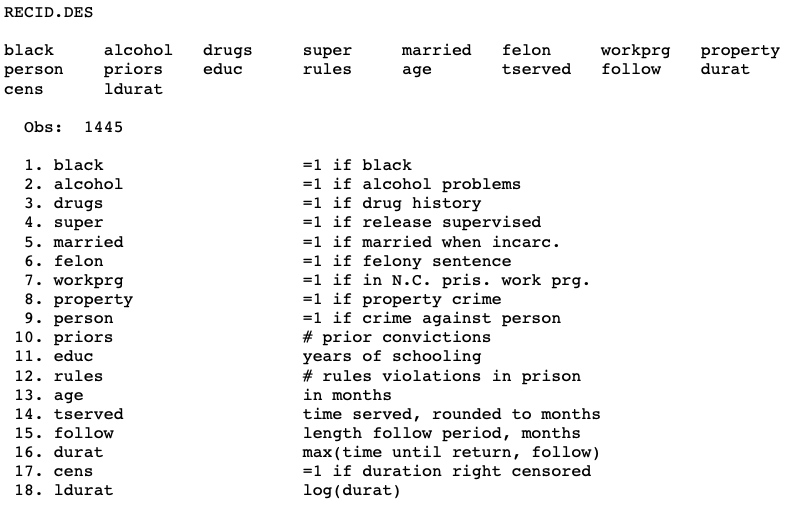
\includegraphics[width=0.53\linewidth]{fig/recid} % requires the graphicx package
		\label{recid}
		\caption{recid.des in Wooldridge's datasets}
	\end{figure} 
\end{frame}
%---------------------------------------------------
\begin{frame}{El modelo de datos truncados}
	\begin{itemize}
		\item Un modelo de datos censurados es aplicable cuando se tiene observaciones de las unidades y la información es parcial; es decir, se tiene información de las variables independientes pero no de la variable $y$.
		\item Usamos Tobit para una solución de esquina (``corner solution outcome'').
		\item Un modelo truncado tiene la característica de excluir (basado en el valor de $y$ ). No se tiene una submuestra aleatoria. Sin embargo, tenemos conocimiento de la regla de exclusión. Esta regla esta determinada si $y$ esta por encima o por debajo de cierto valor (o ``threshold'').   
	\end{itemize}
\end{frame}
%---------------------------------------------------
\begin{frame}{El modelo de datos truncados}
	?`Como surge o se identifica un modelo de datos truncados?
		\begin{itemize}
			\item El investigador presta atención a una submuestra de la población (quizas debido a costos de muestreo, ver Wooldridge). 		   
			\item Hay que enfatizar que la estimación por OLS es eficiente cuando la muestra seleccionada es aleatoria.
		\end{itemize}
	Ejemplos: Hausman y White (1977) usan data de impuestos negativos a la renta como determinante  de las ganancias individuales/familiares. El estudio solo incluía familias con renta 1.5 veces la linea de pobreza.
\end{frame}
%---------------------------------------------------
\begin{frame}{El modelo de datos truncados}
	El modelo de datos truncados puede expresarse de la siguiente manera;
		\begin{equation}
			y=\boldsymbol{x\beta}+u, u \ | \ x, \ \sim Normal(0,\sigma^2)
		\end{equation}
	y el set de datos ($y,x$) es observado solo si $y\ge c_i$ donde el ``threshold'' depende de variables x. Por ejemplo, Haussman y white (1977) definen $c_i$ como el tama\~no de la familia.  
\end{frame}
%---------------------------------------------------
\begin{frame}
	La funcion de distribución gráficamente luce de la siguiente manera;
		\begin{figure}[htbp]
			\hspace*{+1cm} 
			\centering
				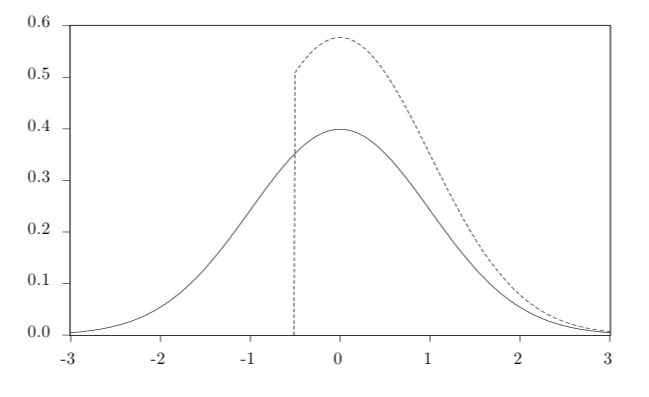
\includegraphics[width=0.70\linewidth]{fig/truncated-model} % requires the graphicx package
			\label{trunc}
			\caption{Source: Chumacero, R, 2003: ``Limited dependent variable'' handout}
		\end{figure} 
\end{frame}
%---------------------------------------------------
\begin{frame}{El modelo de datos truncados}
	La funcion de distribución formalmente luce de la siguiente manera;
		\begin{align}
			g(y|x_i,c_i)=&f(y|x_i\beta,\sigma^2)/F(c_i|x_i,\beta,\sigma^2), y\le c_i
		\end{align}
	donde $f(y|x_i\beta,\sigma^2)$ denota la función de densidad normal y $F(c_i|x_i,\beta,\sigma^2)$ es la función acumulada evaluada en el threshold $c_i$.
	En pocas palabras, se re-pondera dividiendo la función de densidad normal por la acumulada para que la nueva función de densidad sume el valor de uno (1) sobre el dominio de los datos.
	Luego, se toman logs y se estima por ML (es decir, se maximiza la función ($g(y|x_i,c_i$) con los datos observados).
\end{frame}
%---------------------------------------------------
\begin{frame}{!`Vayamos a STATA!}
	Tengamos en cuenta un estudio que tiene el objetivo de modelar el desempe\`no académico como una función de las destrezas de lenguaje (``language skills'') y el tipo de programa en el que los estudiantes se han matriculado. Se requiere analizar a los estudiantes que tengan un desempe\~no mínimo de 40. Tengamos en cuenta la siguiente base de datos en formato STATA:
	\\
	use https://stats.idre.ucla.edu/stat/stata/dae/truncreg, clear
\end{frame}

